\documentclass{article}
\usepackage[T1]{fontenc}
\usepackage{lmodern}
\usepackage{graphicx}
\usepackage{amsmath,amssymb}
\usepackage[a4paper,margin=2cm]{geometry}
\usepackage[absolute,overlay]{textpos}
\setlength{\TPHorizModule}{1mm}
\setlength{\TPVertModule}{1mm}
\usepackage[indonesian]{babel}
\usepackage{hyperref}
\setlength{\emergencystretch}{2em}
% unit: Halaman 16

\begin{document}

% === Halaman 16 (llm) ===

\section*{Masih ingat dengan kasus-kasus ini?}

\vspace{117.61mm}

\begin{itemize}
    \item \textbf{Wikileaks}
    \begin{itemize}
        \item pembocoran dokumen Perang Afghanistan (Juli, 2010)
        \item Pembocoran 400.000 dokumen Perang Irak (Oktober 2010)
        \item Pembocoran kawat diplomatik Amerika Serikat (November 2010)
        \item dll
    \end{itemize}
\end{itemize}

\vspace{20mm}

\textcolor{red}{Julian Assange}, salah satu pendiri situs WikiLeaks.

% deskripsi: Foto Julian Assange dengan latar belakang logo WikiLeaks dan peta dunia
% bbox normalisasi: [0.5870, 0.2060, 0.9840, 0.6020]
\begin{textblock*}{83.37mm}(123.27mm,61.18mm)
\noindent
\includegraphics[width=83.37mm,height=117.61mm]{../../images/llm/page_016_img_01.png}%
\end{textblock*}

% deskripsi: Kliping berita theguardian tentang WikiLeaks dan foto Julian Assange
% bbox normalisasi: [0.1860, 0.6760, 0.4030, 0.9880]
\begin{textblock*}{45.57mm}(39.06mm,200.77mm)
\noindent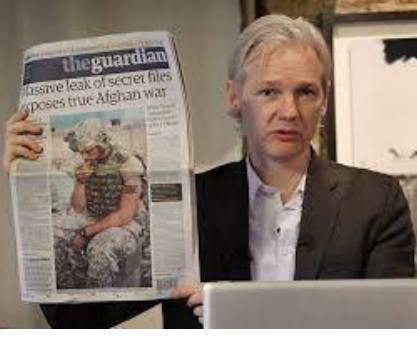
\includegraphics[width=45.57mm,height=92.66mm]{../../images/llm/page_016_img_02.png}%
\end{textblock*}

% deskripsi: Sampul majalah TIME yang menampilkan Julian Assange dengan judul 'Do You Want to Know a Secret?'
% bbox normalisasi: [0.4310, 0.6440, 0.5760, 0.9880]
\begin{textblock*}{30.45mm}(90.51mm,191.27mm)
\noindent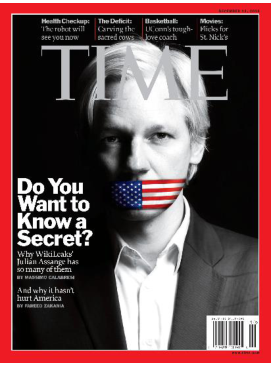
\includegraphics[width=30.45mm,height=102.17mm]{../../images/llm/page_016_img_03.png}%
\end{textblock*}

% deskripsi: Sampul buku atau artikel mengenai Indonesia, WikiLeaks, dan Julian Assange
% bbox normalisasi: [0.7480, 0.6810, 0.8640, 0.9880]
\begin{textblock*}{24.36mm}(157.08mm,202.26mm)
\noindent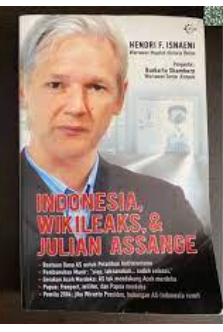
\includegraphics[width=24.36mm,height=91.18mm]{../../images/llm/page_016_img_04.png}%
\end{textblock*}

\end{document}
